\appendix

\chapter{Comandos y mensajes de datos}

%\begin{table}[h]
%	\begin{center}
%		\caption{Códigos de comandos}
%		\label{tabla:comandos_protocolo}
%		\small
%		\begin{tabular}{l|c}
%			\toprule
%			\textbf{Comando} & \textbf{Código}\\
%			\midrule
%			DEVICE\_STATUS & 0x01\\
%			GET\_NETWORK\_STATUS & 0x02\\
%		    GET\_CHILDREN\_AMOUNT & 0x03\\
%			GET\_CHILDREN\_LIST & 0x04\\
%			GET\_LQI\_RSSI & 0x05\\
%			SEND\_DATA\_NODE & 0x06\\
%			DATA\_FROM\_NODE & 0x07\\
%			SET\_RECV\_NODE & 0x08\\
%			SET\_NODE\_OP\_MODE & 0x0A\\
%			START\_MODE\_OPERATION & 0x0B\\
%			STOP\_MODE\_OPERATION & 0x0C\\
%			REQUEST\_DATA\_NODE & 0x0D\\
%			READ\_SENSORS & 0x0E\\
%			READ\_PIN & 0x0F\\
%			READ\_ANALOG & 0x10\\
%			\bottomrule
%		\end{tabular}
%	\end{center}
%\end{table}

\section{Generalidades}

Para el uso de los comandos implementados es necesario considerar las siguientes reglas de funcionamiento: 

\begin{itemize}
	\item Los datos transmitidos mayores a 1 byte (longitud de la trama o direcciones de red, por ejemplo) se transmiten en formato \textit{Big Endian}, es decir, transmitiendo primero el byte más significativo (MSB),
	\item Si el comando especificado no es reconocido por el dispositivo, éste responde con el mensaje UNKNOWN\_COMMAND cuya estructura se muestra en la figura \ref{fig:res_unknown_cmd}, 
	\item Si los parámetros dentro un comando no son reconocidos el dispositivo responde con el mensaje BAD\_PARAMETERS mostrado en la figura \ref{fig:res_bad_parameters}, 
	\item Tanto para UNKNOWN\_COMMAND y BAD\_PARAMETERS el campo de identificador de mensaje es devuelto íntegro para su identificación por el usuario. 
\end{itemize}

\begin{figure}
	\centering
	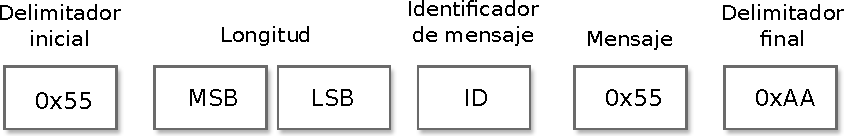
\includegraphics[scale=0.7]{capitulo_3_imgs/res_unknown_cmd.pdf}
	\caption{Mensaje UNKNOWN\_COMMAND}
	\label{fig:res_unknown_cmd}
\end{figure}

\begin{figure}
	\centering
	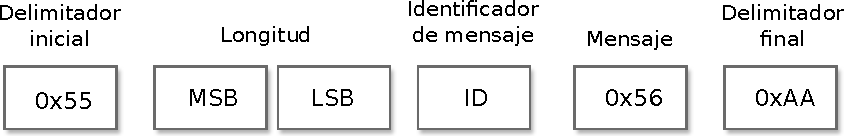
\includegraphics[scale=0.7]{capitulo_3_imgs/res_bad_parameters.pdf}
	\caption{Mensaje BAD\_PARAMETERS}
	\label{fig:res_bad_parameters}
\end{figure}

\section{Información sobre la red}

\subsection{DEVICE\_STATUS}

Código : 0x01

Se utiliza para verificar el funcionamiento del dispositivo comprobando la comunicación mediante la interfaz RS-232. Si el dispositivo está en funcionamiento devuelve el mensaje DEVICE\_UP con un valor de 0x57. Las figuras \ref{fig:cmd_device_status} y \ref{fig:res_device_status} muestran el comando enviado y la respuesta obtenida. 

\begin{figure}[h]
	\centering
	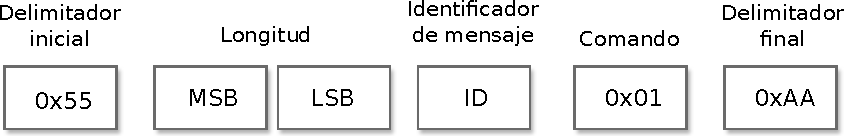
\includegraphics[scale=0.7]{capitulo_3_imgs/cmd_device_status.pdf}
	\caption{Comando DEVICE\_STATUS}
	\label{fig:cmd_device_status}
\end{figure}

\begin{figure}[h]
	\centering
	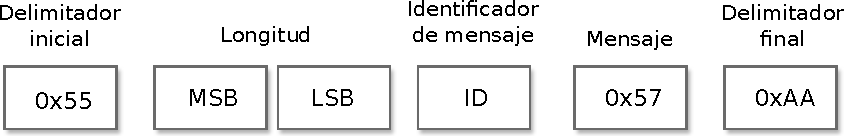
\includegraphics[scale=0.7]{capitulo_3_imgs/res_device_status.pdf}
	\caption{Respuesta al comando DEVICE\_STATUS}
	\label{fig:res_device_status}
\end{figure}

\subsection{GET\_NETWORK\_STATUS}

Código : 0x02

Verifica que la red inalámbrica haya sido iniciada por el dispositivo. Este comando tiene dos respuestas posibles: 1) si la red ha sido iniciada el dispositivo devuelve el mensaje IN\_NETWORK\_STATUS (0x58) junto con el identificador único de la red compuesto por dos bytes y 2) si la red no ha sido iniciada devuelve el mensaje OUT\_NETWORK\_STATUS (0x59). Las figuras \ref{fig:cmd_network_status}, \ref{fig:res1_network_status} y \ref{fig:res2_network_status} muestran la estructura de este comando y sus respuestas.  

\begin{figure}[h]
	\centering
	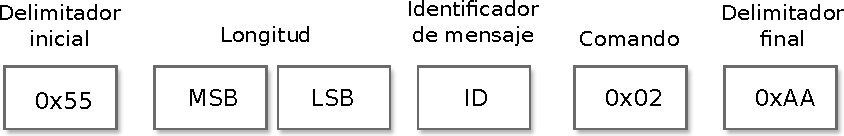
\includegraphics[scale=0.7]{capitulo_3_imgs/cmd_network_status.pdf}
	\caption{Comando GET\_NETWORK\_STATUS}
	\label{fig:cmd_network_status}
\end{figure}

\begin{figure}[h]
	\centering
	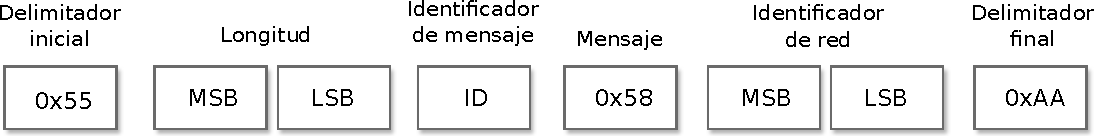
\includegraphics[scale=0.7]{capitulo_3_imgs/res1_network_status.pdf}
	\caption{Respuesta del comando GET\_NETWORK\_STATUS con red iniciada}
	\label{fig:res1_network_status}
\end{figure}

\begin{figure}[h]
	\centering
	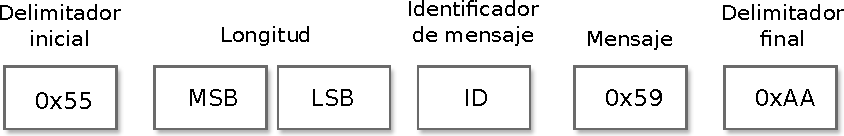
\includegraphics[scale=0.7]{capitulo_3_imgs/res2_network_status.pdf}
	\caption{Respuesta del comando GET\_NETWORK\_STATUS sin red iniciada}
	\label{fig:res2_network_status}
\end{figure}

\subsection{GET\_CHILDREN\_AMOUNT}

Código : 0x03

Obtiene el número de nodos conectados en la red inalámbrica. El número de nodos es devuelto en un byte. En las figuras \ref{fig:cmd_children_amount} y \ref{fig:res_children_amount} se muestra el comando y su respuesta. 

\begin{figure}[h!]
	\centering
	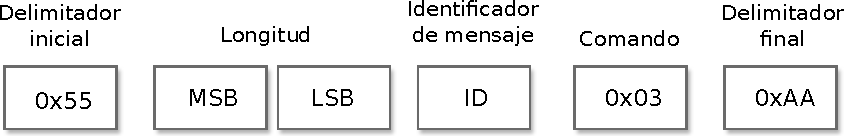
\includegraphics[scale=0.7]{capitulo_3_imgs/cmd_children_amount.pdf}
	\caption{Comando GET\_CHILDREN\_AMOUNT}
	\label{fig:cmd_children_amount}
\end{figure}

\begin{figure}[h!]
	\centering
	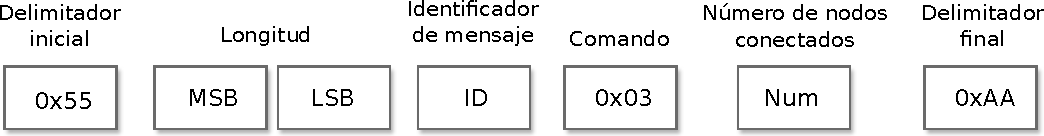
\includegraphics[scale=0.7]{capitulo_3_imgs/res_children_amount.pdf}
	\caption{Respuesta del comando GET\_CHILDREN\_AMOUNT}
	\label{fig:res_children_amount}
\end{figure}


\subsection{GET\_CHILDREN\_LIST}

Código : 0x04

Obtiene la cantidad de nodos conectados al dispositivo junto con las direcciones de red de cada nodo. Cada dirección de red es representada por dos bytes. Las figuras \ref{fig:cmd_children_list} y \ref{fig:res_children_list} muestran el comando y su respuesta. 

\begin{figure}[h]
	\centering 
	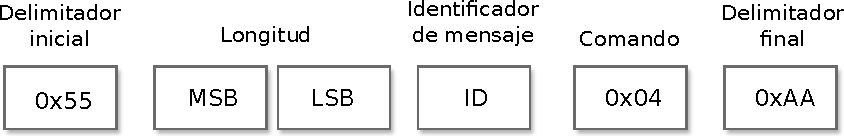
\includegraphics[scale=0.7]{capitulo_3_imgs/cmd_children_list.pdf}
	\caption{Comando GET\_CHILDREN\_LIST}
	\label{fig:cmd_children_list}
\end{figure}

\begin{figure}[h]
	\centering 
	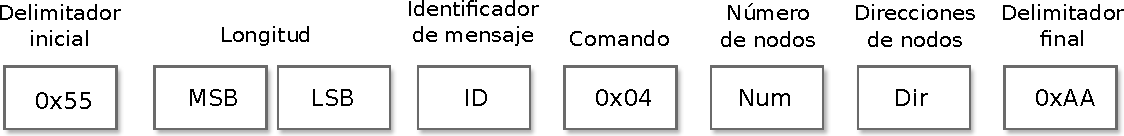
\includegraphics[scale=0.7]{capitulo_3_imgs/res_children_list.pdf}
	\caption{Respuesta del comando GET\_CHILDREN\_LIST}
	\label{fig:res_children_list}
\end{figure}

\subsection{GET\_LQI\_RSSI}

Código : 0x05

Devuelve la calidad del enlace de comunicación (LQI, \textit{Link Quality Indication}) y la calidad de la señal de radio frecuencia (RSSI, \textit{Received Signal Strength Indication}) del dispositivo respecto a un nodo específico, el comando recibe como parámetro dos bytes para la dirección del nodo. La respuesta se compone de dos bytes, en primer lugar se recibe el valor LQI representado por un byte sin signo, en segundo lugar se recibe el valor RSSI representado por un byte con signo. Si la dirección de red proporcionada como parámetro no corresponde a ningún dispositivo activo en la red, los valores LQI y RSSI tienen el valor de cero. 

\begin{figure}[h]
	\centering 
	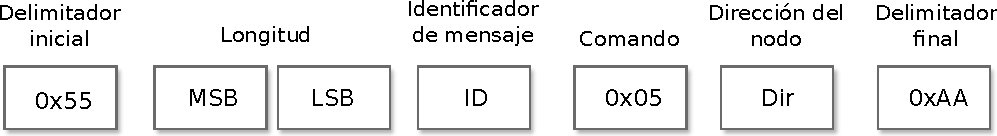
\includegraphics[scale=0.7]{capitulo_3_imgs/cmd_lqi_rssi.pdf}
	\caption{Comando GET\_LQI\_RSSI}
	\label{fig:cmd_lqi_rssi}
\end{figure}

\begin{figure}[h]
	\centering 
	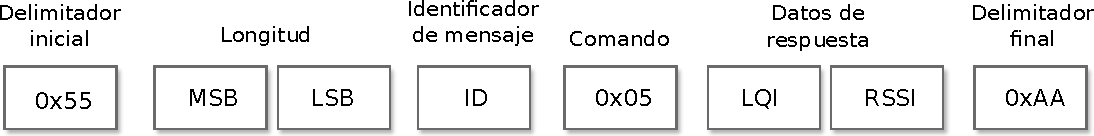
\includegraphics[scale=0.7]{capitulo_3_imgs/res_lqi_rssi.pdf}
	\caption{Respuesta del comando GET\_LQI\_RSSI}
	\label{fig:cmd_children_list}
\end{figure}

\section{Transferencia de datos}

\subsection{SEND\_DATA\_NODE}

Código : 0x06

Envía datos a un nodo especificando su dirección de red. Este comando recibe como parámetro dos bytes para la dirección de red del nodo destino seguido por los datos a ser enviados. De acuerdo a ZigBee el tamaño de los datos no deben superar los 104 bytes. Cuando los datos son enviados hacia la red inalámbrica el dispositivo responde con el mensaje DATA\_SENT (0x5D). En las figuras \ref{fig:cmd_send_node} y \ref{fig:res_send_node} se muestra este comando y su respuesta. 

\begin{figure}[h]
	\centering
	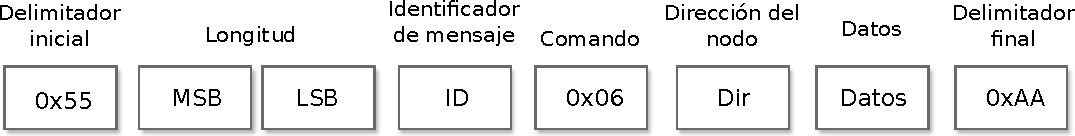
\includegraphics[scale=0.7]{capitulo_3_imgs/cmd_send_data.pdf}
	\caption{Comando SEND\_DATA\_NODE}
	\label{fig:cmd_send_node}
\end{figure}

\begin{figure}[h]
	\centering
	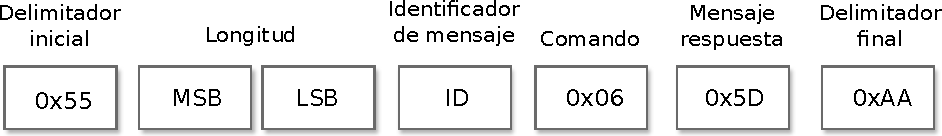
\includegraphics[scale=0.7]{capitulo_3_imgs/res_send_data.pdf}
	\caption{Respuesta al comando SEND\_DATA\_NODE}
	\label{fig:res_send_node}
\end{figure}

\subsection{DATA\_FROM\_NODE}

Código : 0x07

Los datos enviados desde los nodos en la red inalámbrica son devueltos por el dispositivo mediante el mensaje DATA\_FROM\_NODE. Los primeros dos bytes de los datos de este mensaje corresponden a la dirección de red del nodo emisor de los datos, seguido de los datos enviados desde el nodo. La longitud y estructura de esta información depende directamente de la aplicación de la WSN. La figura \ref{fig:res_from_node} muestra la estructura de este comando. 

\begin{figure}
	\centering 
	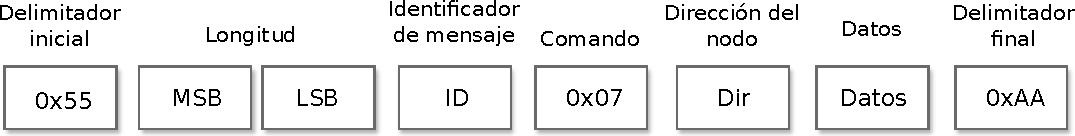
\includegraphics[scale=0.7]{capitulo_3_imgs/res_from_node.pdf}
	\caption{Mensaje de recepción de datos}
	\label{fig:res_from_node}
\end{figure}

\subsection{SET\_RECV\_NODE}

Código : 0x08

Establece el modo de recepción de mensajes desde los nodos en la WSN. Mediante el parámetro ENABLE\_DATA\_RECEPTION (0x5A) todos los mensajes enviados por los nodos son retransmitidos hacia la interfaz RS-232. Con el parámetro DISABLE\_DATA\_--RECEPTION (0x5B) los mensajes recibidos desde la WSN son ignorados. Si se ejecutó el comando correctamente se recibe el mensaje DATA\_RECEPTION\_CHANGED (0x5C). Las figuras \ref{fig:cmd_set_recv} y \ref{fig:res_set_recv} muestran al comando y su respuesta. 

\begin{figure}
	\centering 
	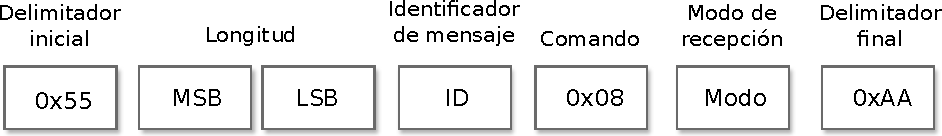
\includegraphics[scale=0.7]{capitulo_3_imgs/cmd_data_recv.pdf}
	\caption{Comando SET\_RECV\_NODE}
	\label{fig:cmd_set_recv}
\end{figure}

\begin{figure}
	\centering
	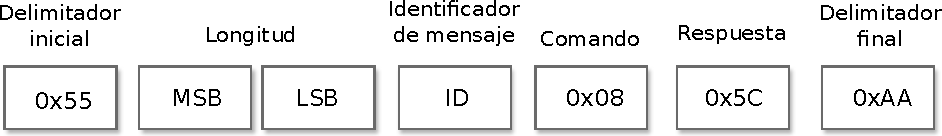
\includegraphics[scale=0.7]{capitulo_3_imgs/res_data_recv.pdf}
	\caption{Respuesta al comando SET\_RECV\_NODE}
	\label{fig:res_set_recv}
\end{figure}

\section{Gestión de nodos}

\subsection{SEND\_COMMAND\_NODE}

Código : 0x0A

Este comando permte enviar comandos y mensajes hacia un nodo en la WSN. Recibe como primer parámetro la dirección de red del nodo destino y como segundo parámetro el comando que se enviará. Los comandos disponibles son : 

\begin{itemize}
	\item SET\_REQUEST\_MODE (0x5D) : Establece el modo REQUEST en el nodo destino, 
	\item REQUEST\_DATA (0x5E) : Solicita datos sensoriales a un nodo en el modo REQUEST,
	\item SET\_SLEEP\_MODE (0x5F) : Establece el modo de operación SLEEP, 
	\item START\_SLEEP\_MODE (0x61) : Inicia el modo de operación SLEEP, 
	\item STOP\_SLEEP\_MODE (0x62) : Detiene el modo de operación SLEEP, 
	\item SET\_RF\_MODE (0x63) : Establece el modo de operación RF, 
	\item START\_RF\_MODE (0x64) : Inicia la operación del modo RF, 
	\item STOP\_RF\_MODE (0x65) : Detiene la operación del modo RF, 
\end{itemize}

Como respuesta a este comando se recibe el mensaje NODE\_COMMAND\_SENT. Las figuras \ref{fig:cmd_set_mode} y \ref{fig:res_set_mode} muestran al comando y su respuesta. 

\begin{figure}
	\centering
	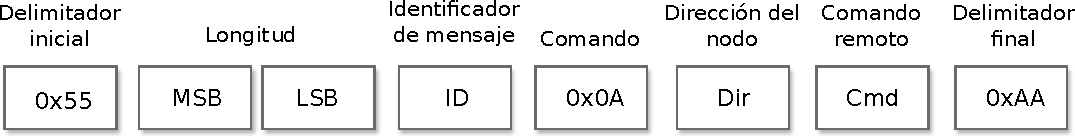
\includegraphics[scale=0.7]{capitulo_3_imgs/cmd_send_command.pdf}
	\caption{Comando SEND\_COMMAND\_NODE}
	\label{fig:cmd_set_mode}
\end{figure}

\begin{figure}
	\centering
	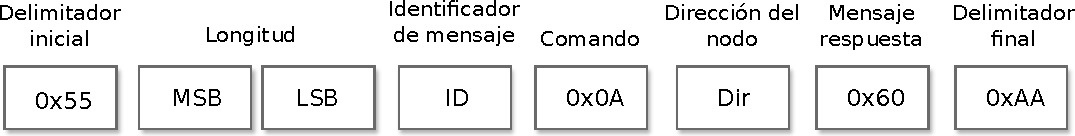
\includegraphics[scale=0.7]{capitulo_3_imgs/res_send_command.pdf}
	\caption{Respuesta al comando SEND\_COMMAND\_NODE}
	\label{fig:res_set_mode}
\end{figure}

\section{Lectura de sensores}

\subsection{READ\_SENSORS}

Código 0x0E

Obtiene información de los sensores conectados al dispositivo. La longitud y estructura de los datos dependerá de la cantidad y tipos de sensores conectados. Las figuras \ref{fig:cmd_read_sensors} y \ref{fig:res_read_sensors} muestran al comando y su estructura. 

\begin{figure}
	\centering
	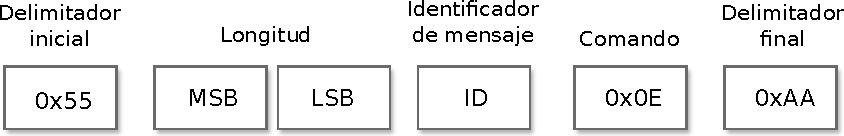
\includegraphics[scale=0.7]{capitulo_3_imgs/cmd_read_sensors.pdf}
	\caption{Comando READ\_SENSORS}
	\label{fig:cmd_read_sensors}
\end{figure}

\begin{figure}
	\centering
	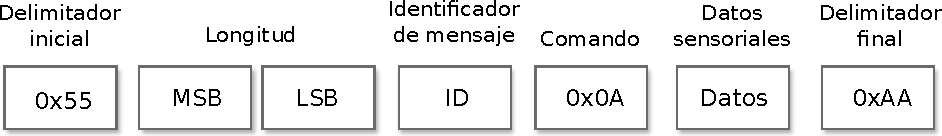
\includegraphics[scale=0.7]{capitulo_3_imgs/res_read_sensors.pdf}
	\caption{Respuesta al comando READ\_SENSORS}
	\label{fig:res_read_sensors}
\end{figure}
